\chapter{Prototype}
\label{ch:prototype}

This chapter will describe implementation of the prototype, and reason for used technologies.

Prototype was created to test if virtual machine technologies are suitable for use in computing platform. HTTP is leveraged as a communication protocol between nodes and the market. BitTorrent protocol is used to distribute said virtual machines to client. Nodes run VirtualBox virtualization software.

Hypothetical network using system described in this thesis is shown in diagram~\ref{f:protomain}. All nodes connect to the server using HTTP, and communicate with one another using BitTorrent~\cite{cohen2008bittorrent} protocol.

\begin{figure}
\centering
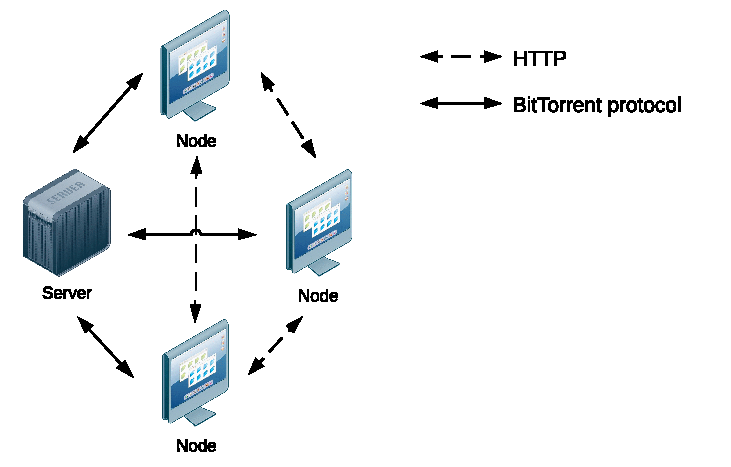
\includegraphics{diagrams/PrototypeMain.pdf}
\caption{Prototype diagram}
\label{f:protomain}
\end{figure}

The prototype implements both client software and the market software, as well as one testing project.

Function specification, that is, the requirements of the prototype, are described in section~\ref{s:funcspec}. Notable implementation details are presented in section~\ref{s:impldet}.

\section{Functional specification}
\label{s:funcspec}

This section presents functional specification of the prototype. It describes responsibilities of both the client and the server software. Communication between them is described, which is done through the \emph{Market API}, as well as method of authentication.

Both server and the client are running in daemon mode, that is, there is no user interface available. User can inspect operation of both programs by looking at the log files. The configuration is being done by editing configuration files with a text editor.

\subsection{Server}

Server is ran by market operator. Server tasks are as follows:

\begin{enumerate}
	\item \label{ps:register} let nodes register themselves,
	\item \label{ps:hand} hand out jobs,
	\item \label{ps:collect} collect results,
	\item \label{ps:measure} measure trust,
	\item \label{ps:track} keep track of project progress.
\end{enumerate}

Task~\ref{ps:register} refers to ability of server to register new nodes and authenticate already registered ones. Node authentication is done with public-key cryptography. Worker uses public/private key pair to to authenticate its request to the server. When connecting for the first time, a permanent record is left in the server's database which is used to recognize that particular client from then on.

"Hand out jobs" task (\ref{ps:hand}) means that server should keep a database of jobs and be able to distribute them to nodes. System presented by this thesis works in a way that the nodes ask for jobs, and the server searches database for suitable job, based on node's trust.

Server should be able to collect results (\ref{ps:collect}) and keep them in a database. By being able to match results with one another and thus confirming them, server is measuring trust (\ref{ps:measure}) of nodes. Those two altogether give the server an ability to decide whether a job is considered finished or not, so the server is able to measure progress (\ref{ps:track}) of the project.

\subsection{Client}

Client is software running on worker computers. Client should be able to:
\begin{enumerate}
	\item \label{cs:auth} authenticate itself to the server,
	\item \label{cs:recv} receive job from the server,
	\item \label{cs:compute} compute received work,
	\item \label{cs:send} send back results of the computation.
\end{enumerate}

(\ref{cs:auth}) means that the client should be able to present itself to the server so both the client can ensure it communicates with entity it think it does, and the server can ensure the client is who it says it is. Methods of doing so are described in section~\ref{s:authentication}.

Receiving jobs from the server (\ref{cs:recv}) consists of two tasks. First is receiving the project, which is the virtual machine and its metadata, from the server. Project files are distributed using BitTorrent technology. After installing and setting the virtual machine up, the client will then ask for job files. Job files are distributed using HTTPS.

When the virtual machine is ready and powered up, job files are sent to the machine and it can start the computation (\ref{cs:compute}). When results are ready, virtual machine sends the results to the client, which then sends them back to the server (\ref{cs:send}).

This process is then repeated. The client asks for next job after finishing one. When there are no jobs left, the client will ask for next project.

The process is also shown in the figure~\ref{f:clientflow}.

\begin{figure}
\centering
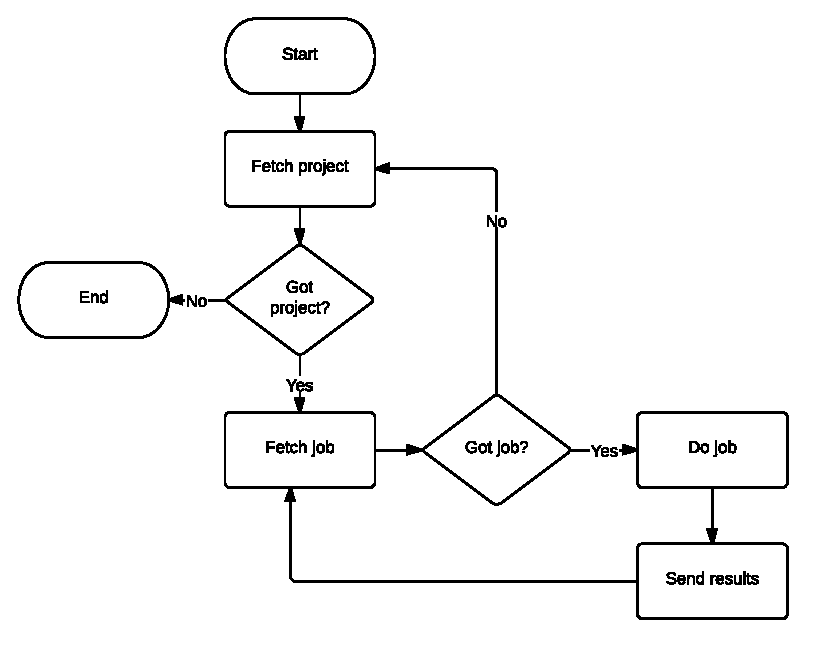
\includegraphics{diagrams/ClientFlowchart.pdf}
\caption{Client flowchart}
\label{f:clientflow}
\end{figure}

\subsection{Authentication}
\label{s:authentication}

Authentication is a two step process. Firstly, the server has to gain trust of the client. The server can do it by either presenting a certificate signed by Certificate Authority, or presenting a self-signed certificate, but transferring the certificate in secure and trusted manner beforehand. For this prototype, we will be working with self-signed certificates, but using the CA is also an implemented option.

Secondly, the server is configured in a way that it will request certificates from the clients. Each client has to generate a key pair and use the private key to authenticate itself when connecting to the server. The certificate fingerprint is used to identify clients. Each client will have different, generated by themselves, key pair, therefore different certificate fingerprint, and due to that, the server is able to identify clients unambiguously using their certificate fingerprints alone.

\section{Architecture}

This section shows how the application is organized. Code for both server and client is separated into modules, using Node.js module system\footnote{Module system is described further in Node.js documentation \url{http://nodejs.org/api/modules.html}}.

Responsibilities of each module will be discussed, and some more significant parts are going to be presented in detail.

Architecture is presented on the figure~\ref{f:arch}. Then, each module's responsibilities are briefly described.

\begin{figure}
\centering
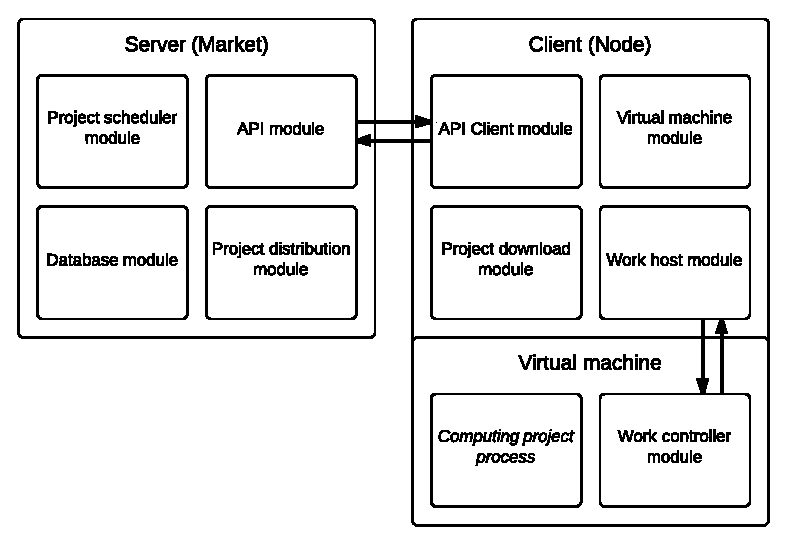
\includegraphics{diagrams/Architecture.pdf}
\caption{Architecture of the prototype. 3 environments can be distinguished: \emph{Server}, \emph{Client}, and \emph{Virtual machine}. Communication between those has been marked with arrows. Only modules with an outgoing arrow can communicate across boundaries of their environments.}
\label{f:arch}
\end{figure}

\subsection{Client}

This section describes modules visible in client environment, pictured on figure~\ref{f:arch}.

\begin{description}

\item[API module] implements very thin client for calling methods exposed by the server. The methods, as well as their purposes, are described in section~\ref{s:cliapi}.

\item[Project download module] is used to fetch project data (virtual machine image and metadata). Internally it uses BitTorrent technology to do that, which allows not only direct transfer from the server, but also peer to peer transfer from other nodes.

\item[Virtual machine module] is used to control virtual machines. VirtualBox\footnote{Virtualbox is a free virtualization product by Oracle, \url{https://www.virtualbox.org/}.} is used as a virtualization engine. This module is used to set up and start virtual machines, when the client starts working on a project.

\item[Work host module] is used to communicate with computing program that is running withing the virtual machine. Because we generally do not place restrictions on what computing programs can be used, special layer has been created in order to exchange data and results with programs. \textbf{Work host module} communicates with \textbf{Work controller module} which is running in virtual machine, and can directly 

\end{description}

\subsection{Server}

This section describes modules visible in server environment, pictured on figure~\ref{f:arch}.

\begin{description}

\item[API module] is used to host an the API for the clients to use. HTTPS is used as the method of communication. Methods implemented within this module are not used internally by server, they are called by the clients instead.

\item[Project scheduler module] is responsible for assigning workers to project and distributing jobs among workers withing a project. For this prototype, assigning to project is done using very simple method. Project scheduler chooses the first project that has undone jobs. Distributing jobs is done using an implementation of algorithm described in section~\ref{s:jobdist}.

\item[Database module] serves as a layer between CouchDB database and the server program.

\item[Project distribution module] is responsible for distributing project files (virtual machines and their metadata). This module prepares a \emph{.torrent} file to return to client. It also starts its own BitTorrent tracker and serves initial (called the \emph{seed}) download.

\end{description}

\section{Market API}
\label{s:cliapi}

This module provides a way for clients to communicate with the server. The communication happens over HTTPS, with use of authentication described in section~\ref{s:authentication}. The module follows REST\footnote{\emph{Representational state transfer}, model for how to build services.} guidelines on how to implement an API.

Client API exposes the following methods that can be remotely called by clients:

\subsection{fetchProject}

\emph{fetchProject} API method is used by clients to discover on what project there will be working on. Result of that call is project id, that will be used internally to fetch project data (distributing projects is explained further in section~\ref{s:torrent_dist}).

This call will result in assigning client to a project when the client is not already in a project. Otherwise, current project id is returned, and no changes are made to the client. So this call is not only used to request the project, but also to discover what project is the client working on, after it starts.

\subsection{fetchJob}

\emph{fetchJob} method is used to discover what job client will be working on. Result of this call is job id, which is used later to fetch job data, and to send results back (with \emph{sendResult} method).

This call results in finding new work for client only when client has finished previous job (or has not fetched a job in their project yet). There is no way of changing job or aborting one. When client already has a job and calls \emph{fetchJob}, job id of current job is returned, and no changes are made to the client. \emph{fetchJob} is used when client starts (along with \emph{fetchProject}) to start working, whether it will result in getting new project or new job (or both), or continuing where the client has left.

\subsection{sendResult}

\emph{sendResult} is called by client when their computation is finished and results are ready to be sent back. Results are sent as a binary data and the server does not care about the format. This is done to ensure maximum flexibility as far as projects are concerned. After receiving, initial correctness of the is computed, which is the reliability of the node. 

Hash of the data (using SHA1) is computed. We can now easily compare newly received result to results that have been handed in before. For each of the results that are equal (hash values match), \emph{total score} is increased. Job record keep \emph{total score} for each unique result received, by mapping it to the hash value. When unique result's score exceeds $1$, the job is marked as \emph{done}.

If there is are no prior results with hash matching, the raw data is also saved to the database.

Example of completing results is shown in figure~\ref{f:sendresultsex}.

After sending the result, client should ask for another job, using \emph{fetchJob} method.

\begin{figure}
\centering
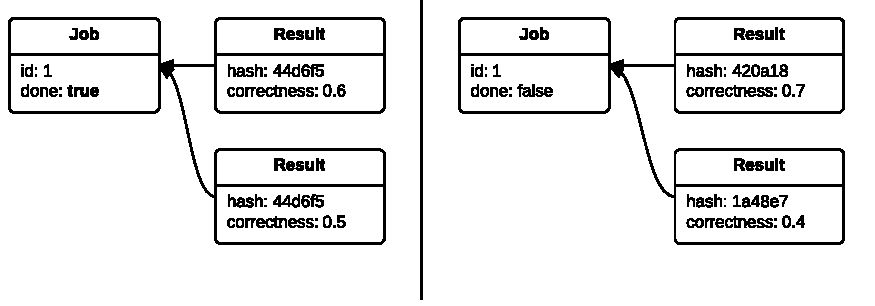
\includegraphics{diagrams/SendResultsExample.pdf}
\caption{Two examples of job with two results. Job in example on the left is marked as \emph{done}, because sum of correctness of results exceeds $1$. Example on the right shows undone job, because even though correctness exceeds $1$, the nodes has not agreed on the results (the hash differs).}
\label{f:sendresultsex}
\end{figure}

\section{Implementation details}
\label{s:impldet}

\subsection{Distribution and download modules}
\label{s:torrent_dist}

\emph{Distribution module} on the server, and corresponding \emph{download module} on the client, are used to to effectively transfer project files (stored on the server) to the client. BitTorrent protocol is used to save bandwidth and speed up the transfer.

\emph{node-torrent}\footnote{https://github.com/zapu/node-torrent} library is used by both modules. It is used to parse \emph{.torrent} files. \emph{node-torrent} is also a BitTorrent client. Important fact is that the server also runs a BitTorrent client and takes part in BitTorrent data exchange. In theory, after the first worker of the project downloads the project data, server could stop serving it. But in practice, it is better for the network if the server remains active.

Download module uses \emph{node-torrent} module to provide ability to use BitTorrent protocol to fetch project data. Project data consists of VirtualBox virtual machine files. The module export one function, which given the \emph{.torrent} file, will proceed with the download and call back when it is completed.

The \emph{.torrent} contains all the metadata necessary to download and verify data, which in our case is virtual machine image. Also included are URL addresses of torrent trackers, which serve as a "meeting point" for nodes, in case node discovery via Distributed Hash Table fails.

Figure~\ref{f:clientprojdownload}~shows how all three modules (\emph{Market API}, \emph{Download module}, and \emph{Virtual machine module}) are used to fetch virtual machine with project data from Market. First an API call is made to acquire \emph{.torrent} file. Then, \emph{Download module} is used to connect to peers and fetch torrent data to local file system. The \emph{virtual machine module} then registers the downloaded virtual machine. This action makes it ready to use.

\begin{figure}
\centering
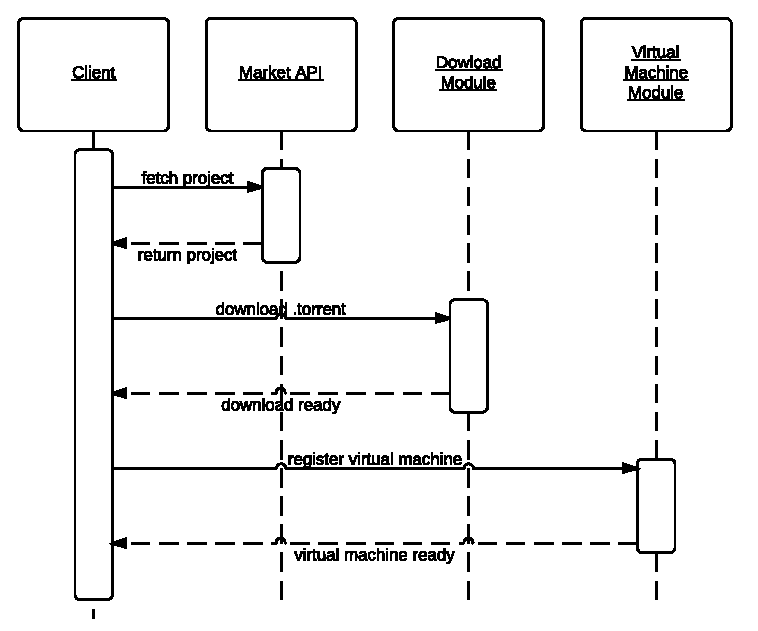
\includegraphics{diagrams/ClientProjectDownload.pdf}
\caption{Sequence diagram showing how virtual machine is fetched from Market and then registered within Virtual machine module (described in section~\ref{s:c_vm_mod}).}
\label{f:clientprojdownload}
\end{figure}

\subsection{Virtual machine module}

\label{s:c_vm_mod}

\begin{comment}
http://www.virtualbox.org/manual/ch08.html
\end{comment}

Virtual machine module is used to launch the project virtual machine using VirtualBox virtualizer. Internally, it uses \emph{VBoxManage}\footnote{VBoxManage is an utility provided by Virtual Box. \url{http://www.virtualbox.org/manual/ch08.html}} for operating on Virtual Box. \emph{VBoxManage} provides functionality, such as

\begin{description}
\item[list] to list virtual machines,
\item[import] to import virtual machine file,
\item[unregistervm] to remove already added virtual machine,
\item[controlvm] to power off or reset virtual machine,
\item[startvm] to start virtual machine.
\end{description}

The module is mostly a wrapper over \emph{VBoxManage} command line utility. The following are code listings\footnote{Consult \url{http://maxtaco.github.io/coffee-script/} website for syntax reference.} for implementations of the \emph{list} wrapper and \emph{import} wrapper. \emph{list} wrapper not only calls \emph{VBoxManage}, but also parses the output to produce JavaScript array of objects, instead of flat text.

\begin{lstlisting}[caption=Function wrapping \emph{vm list} method.]
vm_list = (what, autocb) ->
  await exec "#{$.VBoxManage} list #{what}", 
    defer error, stdout, stderr

  throw error if error

  results = []

  for line in stdout.split("\n")
    matches = line.match /"(.*)" \{([0-9a-f\-]*)\}/
    if matches?
      results.push 
        name: matches[1]
        guid: matches[2]

    return results
\end{lstlisting}

\begin{lstlisting}[caption=Function wrapping \emph{vm import} method.]
import_vm = (path, name, autocb) ->
  await exec "#{$.VBoxManage} import #{path} --vsys 0 --vmname #{name}",
    defer error, stdout, stderr

  throw error if error
\end{lstlisting}

\subsection{Work module}

Work module is used to communicate with project executable running within virtual machine. It works by creating a HTTP server in local network (network between the virtual machine and the host operating system). The project then makes requests to this web server, receiving work items, until there is no more work left. Sequence diagram in figure~\ref{f:clientseq} shows an example situation where work is fetched from the market (\emph{MarketAPI}), a virtual machine is powered on (via \emph{VM Module}) and data is exchanged with computing program on the virtual machine using \emph{work module} (\emph{Virtual machine project} on the diagram).

\begin{figure}
\centering
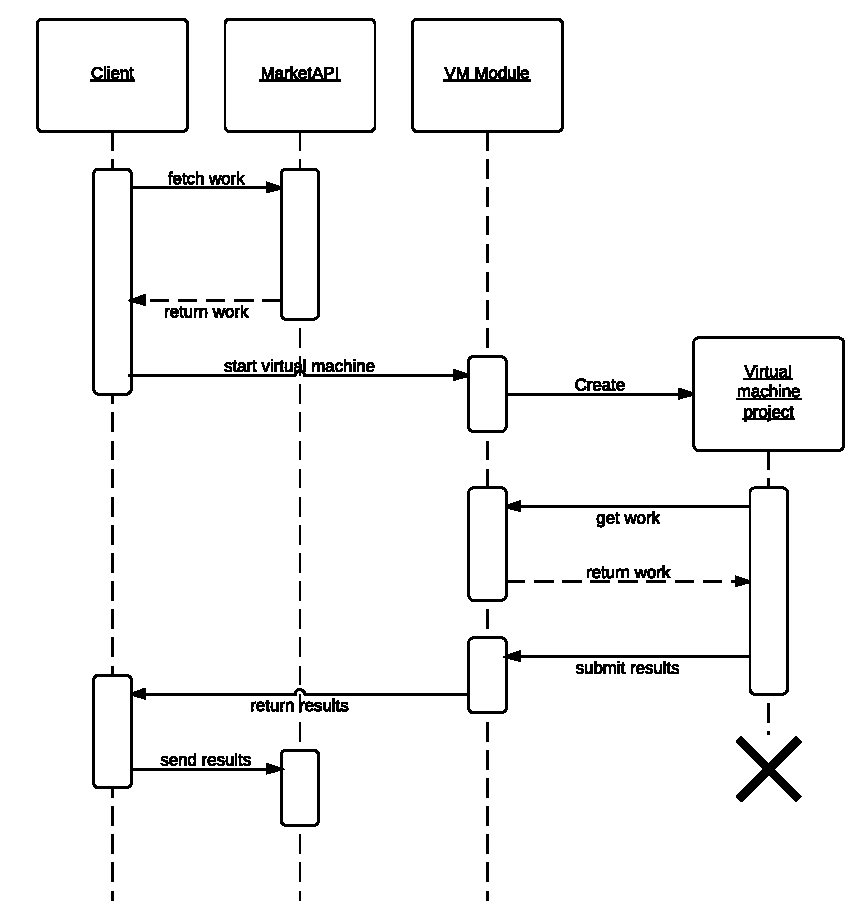
\includegraphics{diagrams/ClientSequence.pdf}
\caption{Sequence diagram showing interaction between client, Market module, Virtual machine module and Work module.}
\label{f:clientseq}
\end{figure}

The protocol is based on HTTP and uses simple GET and POST methods. First, the guest OS is able to ask for job data when it's done setting itself up, using GET request. Then, after computation finishes, it does a POST request to send job computation results. It is important to note that the communication is one-sided as far as data exchange is considered - guest OS initiates both transferring job data and transferring job results. The protocol, however, describes one action in which the host OS initiates communication. It is the "PING" mechanism, which is used to check whether guest OS machine is still computing, and has not crashed because of any critical unforeseen failure. 

The "PING" mechanism is implemented using HEAD requests. Guest OS is expected to host a HTTP server responding to HEAD requests if computing is being performed without problems. Host OS will periodically perform the requests. If any times out, that means the application is not performing computation at the time and has probably hung. Guest OS is to be restarted when such behavior is detected. Guest OS has to ensure that it will not reply to this request when computation is interrupted.

\subsection{Database}

CouchDB\footnote{http://couchdb.apache.org/} is used as database engine. CouchDB is an open source NoSQL database that uses JSON\footnote{Javascript Object Notation, http://www.json.org/} documents. It also allows storing files. Ability to store binary data and the fact that it operates on Javascript Objects made it feasible to use this database engine in the prototype.

Prototype uses \emph{cradle}\footnote{https://github.com/flatiron/cradle} Node.js library to connect to CouchDB.

In the prototype, we use two types of documents. One for projects and one for jobs.

\subsubsection{Project documents}

Example project document looks as follows:

\begin{lstlisting}[caption=Project document in JSON format.]
{
   "_id": "737c253d85f094381717159a55007268",
   "_rev": "9-7cd64eba7ca90f2a05dca23e4f5e2ae1",
   "type": "project",
   "participants": [
       "a26ef8e8165be078e324f62629575c37f69f2d83",
       "d0efb2a9fd86ef76822f72ad245e0565ed299263",
   ],
   "_attachments": {
       "program": {
           "content_type": "application/octet-stream",
           "revpos": 2,
           "digest": "md5-G+EYqBT17Z3W04UIGiYA2w==",
           "length": 402938880,
           "stub": true
       }
   }
}
\end{lstlisting}

\begin{description}
\item[\_id and \_rev] are internal CouchDB fields, representing document unique id and revision id.
\item[type] is always set to "project", defines document type.
\item[participants] is the list of all nodes participating in the project. Each node is represented by hash of its public key. For more information about using keys for this, refer to section~\ref{s:authentication}.
\item[\_attachments] is internal CouchDB field for attachment. Each \emph{project} document has one attachment called "program", in which virtual machine image is stored.
\end{description}

\subsection{Job document}

Example job document looks as follows:

\begin{lstlisting}[caption=Job document in JSON format.]
{
   "_id": "737c253d85f094381717159a55007cfa",
   "_rev": "7-77219fafaabff4263e8cb8e869bd39d8",
   "type": "work",
   "project_id": "737c253d85f094381717159a55007268",
   "results": [
       {
           "node": "a26ef8e8165be078e324f62629575c37f69f2d83",
           "score": 0.006756688654422763,
           "hash": "1fb021c0a2a953d76a20f064f4a0b8ec6e307687"
       },
       {
           "node": "d0efb2a9fd86ef76822f72ad245e0565ed299263",
           "score": 0.19533568197607692,
           "hash": "1fb021c0a2a953d76a20f064f4a0b8ec6e307687"
       }
   ],
   "requests": [
   ],
   "_attachments": {
       "1fb021c0a2a953d76a20f064f4a0b8ec6e307687": {
           "content_type": "application/octet-stream",
           "revpos": 4,
           "digest": "md5-w0Qk2F4ACtibM7KshWfutQ==",
           "length": 8212,
           "stub": true
       },
       "data": {
           "content_type": "application/octet-stream",
           "revpos": 2,
           "digest": "md5-Vb+Jcqx9ZKMFlFY6jbQg1Q==",
           "length": 25,
           "stub": true
       }
   }
}
\end{lstlisting}

\begin{description}
\item[\_id and \_rev] are internal CouchDB fields.
\item[type] is always set to "work" (not "job" due to backwards compatibility reasons).
\item[results] is array of result objects. Each object has following notation:
  \begin{description}
  \item[node] is the id of node sending the result.
  \item[score] is correctness of node when sending the result.
  \item[hash] is result of hash function applied to result data. It is used to compare the results (if their hash matches, we assume the results are identical).
  \end{description}
 \item[requests] is an array that holds ids of nodes that has been sent the job and the market is awaiting their results. It is the equivalent of \emph{AssumedResult} from the simulator (\ref{s:simdesign}).
 \item[\_attachments] is the field for attachments. Attachments for this type of document are results and the job data itself. Only one copy of the results is stored per hash (so we do not store identical binary data objects multiple times).
\end{description}

Each time a node sends its result, we add an item to \emph{results} array. Then, if no other result exists with the same hash, we also store attachment with result data.

\section{Test project}

The prototype comes with an example computing project. The project runs on Node.js platform and is installed under Arch Linux\footnote{https://www.archlinux.org/}. Virtual machine image for the project is 400MB in size.

\subsection{The problem}

The project computes Cunningham chains~\cite{andersen2005cunningham}, which are sequences of prime numbers, that follow that

\begin{equation}
p_i = 2^{i-1}p_1 + (2^{i-1}-1)
\end{equation}

Jobs for the project are simply pairs of numbers, first number \emph{from} to start the search, and the second number where the search should end.

\begin{lstlisting}[caption=Javascript code for searching Cunningham chains.]
checkChain = function(num) {
  if(!isPrime(num))
    return null;

  var list = [ num ];
  var coeff = 2;
  for(;;) {
    var val = coeff * num + coeff - 1;
    if(!isPrime(val)) {
      return list.length > 1 ? list : null;
    }

    coeff *= 2;
    list.push(val);
  }
}

module.exports = function(work) {
  var results = [];
  for(var i = work.from; i <= work.to; i++) {
    var chain = checkChain(i);
    if(chain) {
      results.push(chain);
      console.log("Got chain", chain);
    }
  }
  return results;
}
\end{lstlisting}

\subsection{Test run}

The prototype is ran from the console and informs user about its progress using \emph{standard output}. Right after running the client applications, user sees:

\begin{lstlisting}[caption=Standard output of client application.]
Working on project 59ccf0abd01ab22454c428d78b007a5d
Downloading project virtual machine files...
  downloading [===================] 100% 0.0s

Download complete
Download completed, setting up VM...
Importing VM
Starting VM
\end{lstlisting}

Which shows that client has properly registered in project, managed to download virtual machine and set it up within VirtualBox.

We can inspect that the machine is running by using VirtualBox GUI (shown on image~\ref{f:vboxgui}).

\begin{figure}
\centering
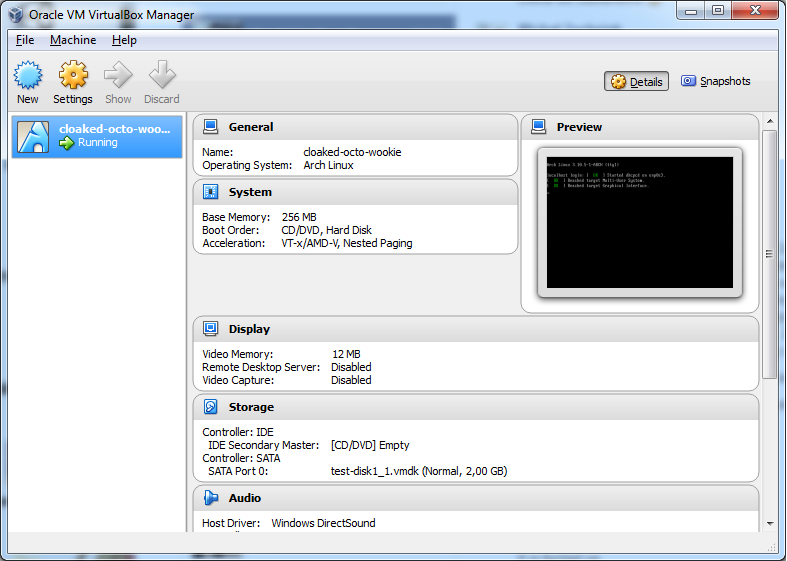
\includegraphics[width=\textwidth]{images/virtualbox.png}
\caption{VirtualBox GUI showing imported and running virtual machine.}
\label{f:vboxgui}
\end{figure}

Then, the client will receive work from the server, send it to the virtual machine, and wait for computation results. This will be repeated until the program is stopped, or there is no more work left for this particular client.

\begin{lstlisting}[caption=Standard output of client application.]
got work 1
Waiting for results...
Submitting work...
Done
...
Done
{ code: 404, body: 'No more work' }
Powering down and removing VM
\end{lstlisting}